\section{Referencia de la Estructura expr}
\label{structexpr}\index{expr@{expr}}
Clase de almacenamiento de raiz de un arbol de expresiones en el AST.  


{\tt \#include $<$ast.h$>$}

Diagrama de colaboraci\'{o}n para expr:\begin{figure}[H]
\begin{center}
\leavevmode
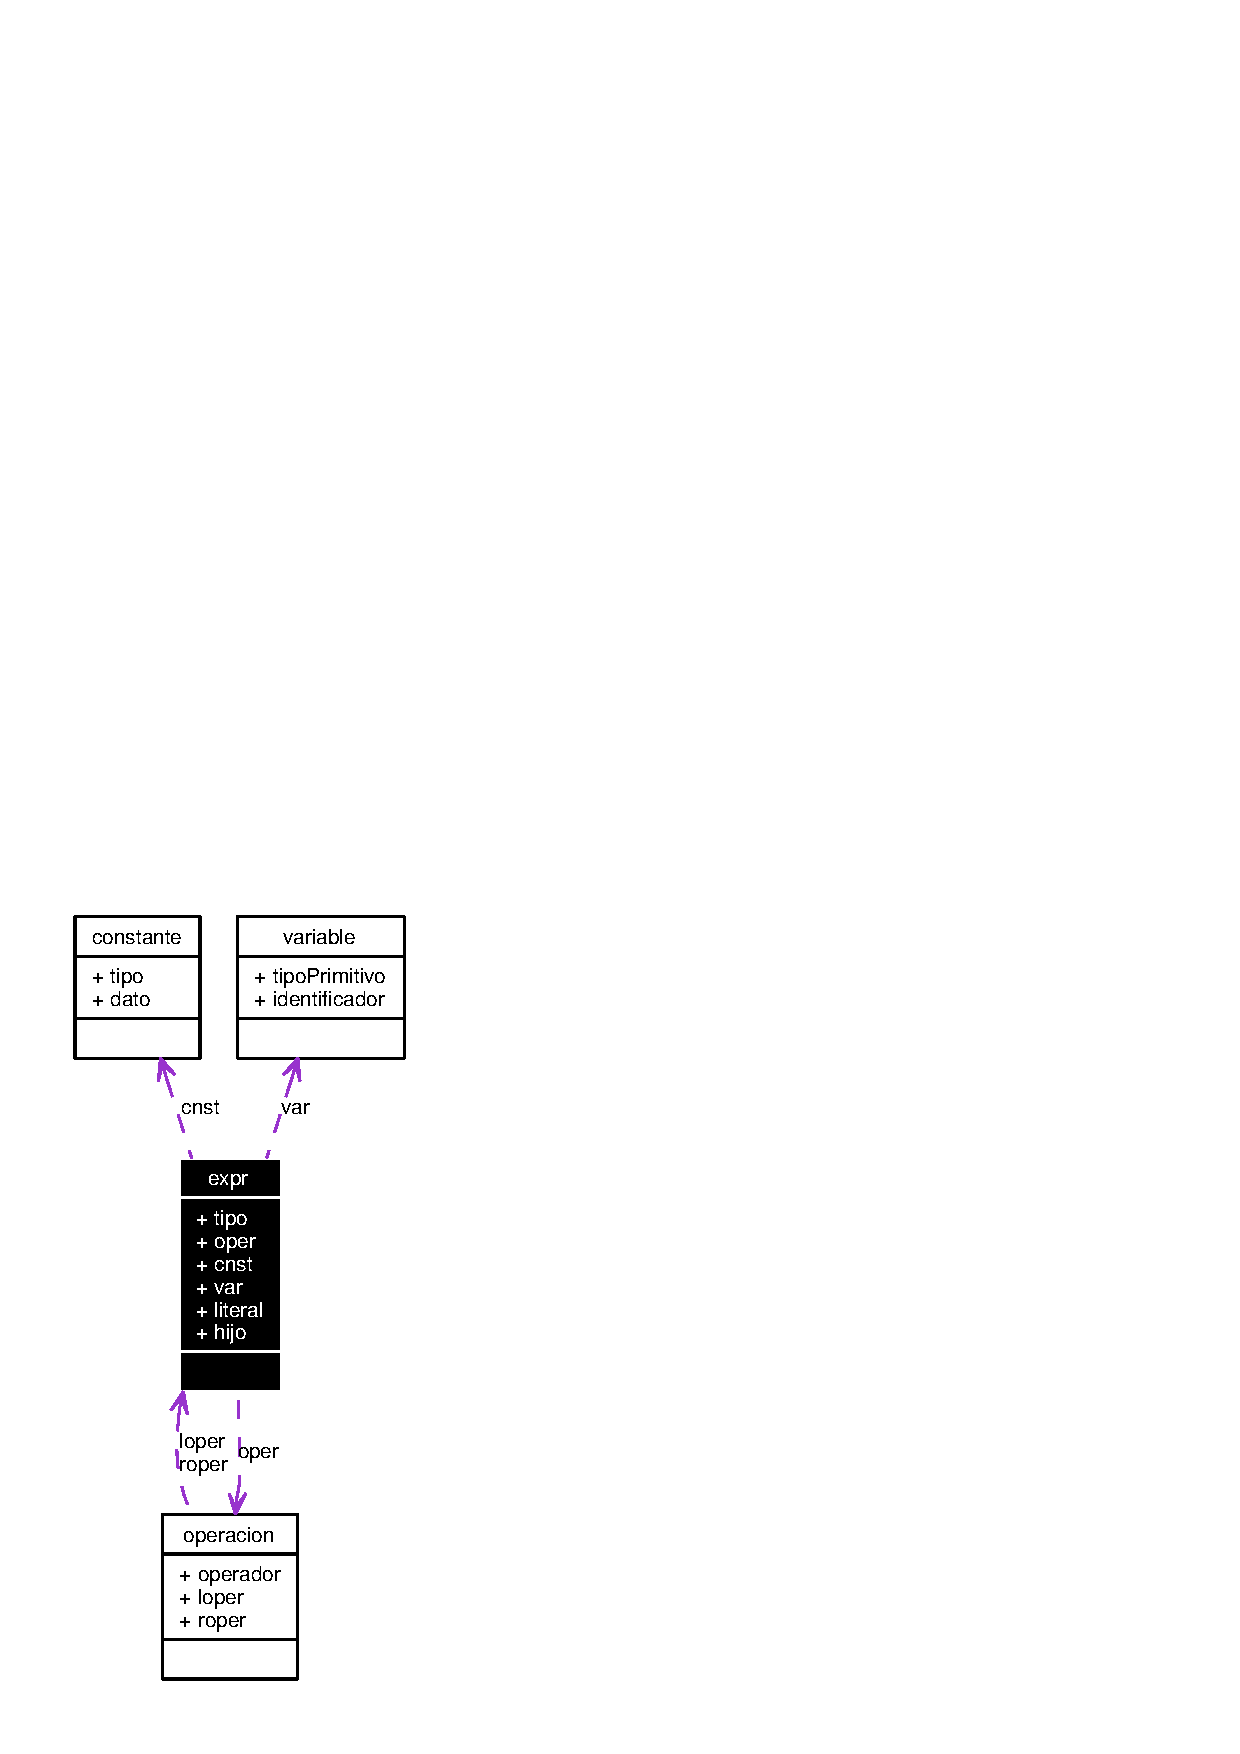
\includegraphics[width=97pt]{structexpr__coll__graph}
\end{center}
\end{figure}
\subsection*{Atributos p\'{u}blicos}
\begin{CompactItemize}
\item 
int {\bf tipo}
\begin{CompactList}\small\item\em Tipo de expresion. \item\end{CompactList}\item 
\begin{tabbing}
xx\=xx\=xx\=xx\=xx\=xx\=xx\=xx\=xx\=\kill
union \{\\
\>{\bf operacion} $\ast$ {\bf oper}\\
\>{\bf constante} $\ast$ {\bf cnst}\\
\>{\bf variable} $\ast$ {\bf var}\\
\>char $\ast$ {\bf literal}\\
\} {\bf hijo}\\

\end{tabbing}\begin{CompactList}\small\item\em Puntero a dato correspondiente. \item\end{CompactList}\end{CompactItemize}


\subsection{Descripci\'{o}n detallada}
Clase de almacenamiento de raiz de un arbol de expresiones en el AST. 



Definici\'{o}n en la l\'{\i}nea 205 del archivo ast.h.

\subsection{Documentaci\'{o}n de los datos miembro}
\index{expr@{expr}!cnst@{cnst}}
\index{cnst@{cnst}!expr@{expr}}
\subsubsection{\setlength{\rightskip}{0pt plus 5cm}{\bf constante}$\ast$ {\bf expr::cnst}}\label{structexpr_o2}




Definici\'{o}n en la l\'{\i}nea 209 del archivo ast.h.\index{expr@{expr}!hijo@{hijo}}
\index{hijo@{hijo}!expr@{expr}}
\subsubsection{\setlength{\rightskip}{0pt plus 5cm}union \{ ... \}  {\bf expr::hijo}}\label{structexpr_o5}


Puntero a dato correspondiente. 



Referenciado por borrar\-Expresion(), evaluar\-Expresion(), insertar\-Cadena(), y insertar\-Expresion().\index{expr@{expr}!literal@{literal}}
\index{literal@{literal}!expr@{expr}}
\subsubsection{\setlength{\rightskip}{0pt plus 5cm}char$\ast$ {\bf expr::literal}}\label{structexpr_o4}




Definici\'{o}n en la l\'{\i}nea 211 del archivo ast.h.\index{expr@{expr}!oper@{oper}}
\index{oper@{oper}!expr@{expr}}
\subsubsection{\setlength{\rightskip}{0pt plus 5cm}{\bf operacion}$\ast$ {\bf expr::oper}}\label{structexpr_o1}




Definici\'{o}n en la l\'{\i}nea 208 del archivo ast.h.\index{expr@{expr}!tipo@{tipo}}
\index{tipo@{tipo}!expr@{expr}}
\subsubsection{\setlength{\rightskip}{0pt plus 5cm}int {\bf expr::tipo}}\label{structexpr_o0}


Tipo de expresion. 



Definici\'{o}n en la l\'{\i}nea 206 del archivo ast.h.

Referenciado por borrar\-Expresion(), evaluar\-Expresion(), insertar\-Cadena(), y insertar\-Expresion().\index{expr@{expr}!var@{var}}
\index{var@{var}!expr@{expr}}
\subsubsection{\setlength{\rightskip}{0pt plus 5cm}{\bf variable}$\ast$ {\bf expr::var}}\label{structexpr_o3}




Definici\'{o}n en la l\'{\i}nea 210 del archivo ast.h.

La documentaci\'{o}n para esta estructura fu\'{e} generada a partir del siguiente archivo:\begin{CompactItemize}
\item 
/media/docs/progra/c++/compiladores1/proy2/godzilla/src/{\bf ast.h}\end{CompactItemize}
